In order to arrive at informed and assessable observability design decisions, we need to be able to quantify their effectiveness. Observability serves as a necessary precursor for measuring many other system qualities, such as performance \cite{Ahmed_EffectivenessOfAPM_2016} or cost \cite{Kuhlenkamp_Costradamus_2017}, but observability itself is very challenging to quantify~\cite{Tamburri_MVCObservability_2018}. 
Its effectiveness is intricately connected with the very aspects it aims to capture. 
In this work, we look at observability for the specific purpose of reliability assurance, i.e., the process of ensuring that the system is running despite failures occurring.

Reliability assurance centers around two key metrics: (1) mean-time-to-failure / mean-time-between-failures ($MTTF / MTBF$) and (2) mean-time-to-restore ($MTTR$). $MTTR$ can be further divided into (2.1) mean-time-to-detect ($MTTD$) and (2.2) mean-time-to-repair ($MTTRepair$). 
The goal of maintaining a high $MTTF$ mostly falls beyond the domain of observability and instead relies on thorough testing. $MTTR$, conversely, is influenced by the presence of observability measures. 

Still, $MTTD$ and $MTTR$-like metrics aren't specific to observability mechanisms but apply to the entire operation process, including any other fault-tolerance mechanisms implemented. They serve to track the long-term effect of reliability measures and of reliability teams but are too coarse and can be influenced by many different overlapping factors.
For example, they do not indicate whether a failure could have been detected earlier or at less cost with a different observability configuration. To arrive at a systematic method for observability design decisions, we need to measure the impact of configuration and instrumentation decisions. Hence, we need to broaden our perspective beyond time-based process metrics. In the following, we propose a first set of fine-grained metrics as a basis of such a systematic method. 

\subsection{Concept: Fault Observability Metrics}\label{sec:metrics}
To arrive at testable and explicit metrics for observability design decisions, we restrict our scope to the visibility of faults, or what we call \textbf{fault visibility}\cite{Borges_TracingServerless_2021}. Fault visibility can be defined as the degree to which the data produced during the occurrence of a specific fault is distinct enough from normal operation to trigger a fault detection mechanism. 
Intuitively, faults that produce very distinct data are easier and faster to troubleshoot. 
For \textbf{fault visibility}, we consider a set of faults $ F = \{f_1, f_2, ..., f_l\}$, a set of observability metrics or traces $M = \{m_{1},m_{2},...,m_{n}\}$ and a detection mechanism $d$. A fault $f$ can be considered visible in metric $m$ if the data recorded during the occurrence of the fault, represented by the time interval $[t_{0} - t_{1}]$, is significantly different from the data recorded under normal conditions, in time interval $[t_{\text{-}1} - t_{0}[$, and thus detected by detection mechanism $d$. Refer to \Cref{fig:faultmodel}(A) for a visual representation of these time intervals. 
As modeled in section \ref{sec:model1}, the detection mechanism can be of different types, e.g., a pre-trained classifier. We consider fault $f$ visible in metric $m$ if detection method $d$ is able to meet its detection threshold and detect the fault. If the detection mechanism is not able to detect the fault, it suggests that either (i) metric $m$ is unsuitable to detect $f$ (ii) the parameters of metric $m$ are not set appropriately or (iii) the function parameters of the detection mechanism $d$ are not tuned correctly. Fault visibility for fault $f$ in metric $m$ through detection mechanism $d$ can thus be defined as
\begin{equation}
    v_{f,m,d}=\left\{
    \setlength{\arraycolsep}{0.2cm}
    \begin{matrix} 
     1 & \quad  DF(m_{t}) > \alpha \\  
     0 & \quad \text{otherwise}  \\ 
    \end{matrix}\right.
\end{equation}
where $DF$ represents the detection function of $d$, $\alpha$ the configured threshold and $m_t$ a subset of observations of m for time $t$. 


The visibility score can be determined for each fault and metric pair, allowing us to assess the impact of individual faults on specific metrics given their current configuration. 
However, these individual scores are not able to provide a comprehensive and generalized understanding of the observability of the system as a whole. To accomplish this, we can construct aggregate or composite scores. We propose two composite scores: fault coverage and overall fault observability. 
\textbf{Fault coverage} shows the degree to which a fault $f$ is visible across the set of different collected metrics $M$. We define it as the ratio between the number of collected metrics and a number of metrics where fault $f$ is visible. If a fault is not visible in any metric of the system, it implies that this fault is not covered by the system's observability, and thus the fault coverage for fault $f$ is 0.
\begin{equation}
    FC_{f,d}=\frac{1}{n}\sum_{i = 1}^{n} v_{f,m_{i},d}
\end{equation}

Lastly, the \textbf{overall fault observability} shows the ratio between the theoretically observable faults versus the faults that were actually observed or detected by detection mechanism $d$. This ratio can improve over time, as developers add more metrics to the instrumentation, or tune the configuration. It can then be defined as
\begin{equation}
    OFO_{d}= \frac{1}{l}\sum_{i = 1}^{l} 1_{\{FC_i > 0\}}
\end{equation}

\begin{figure}[t]
    \centering
    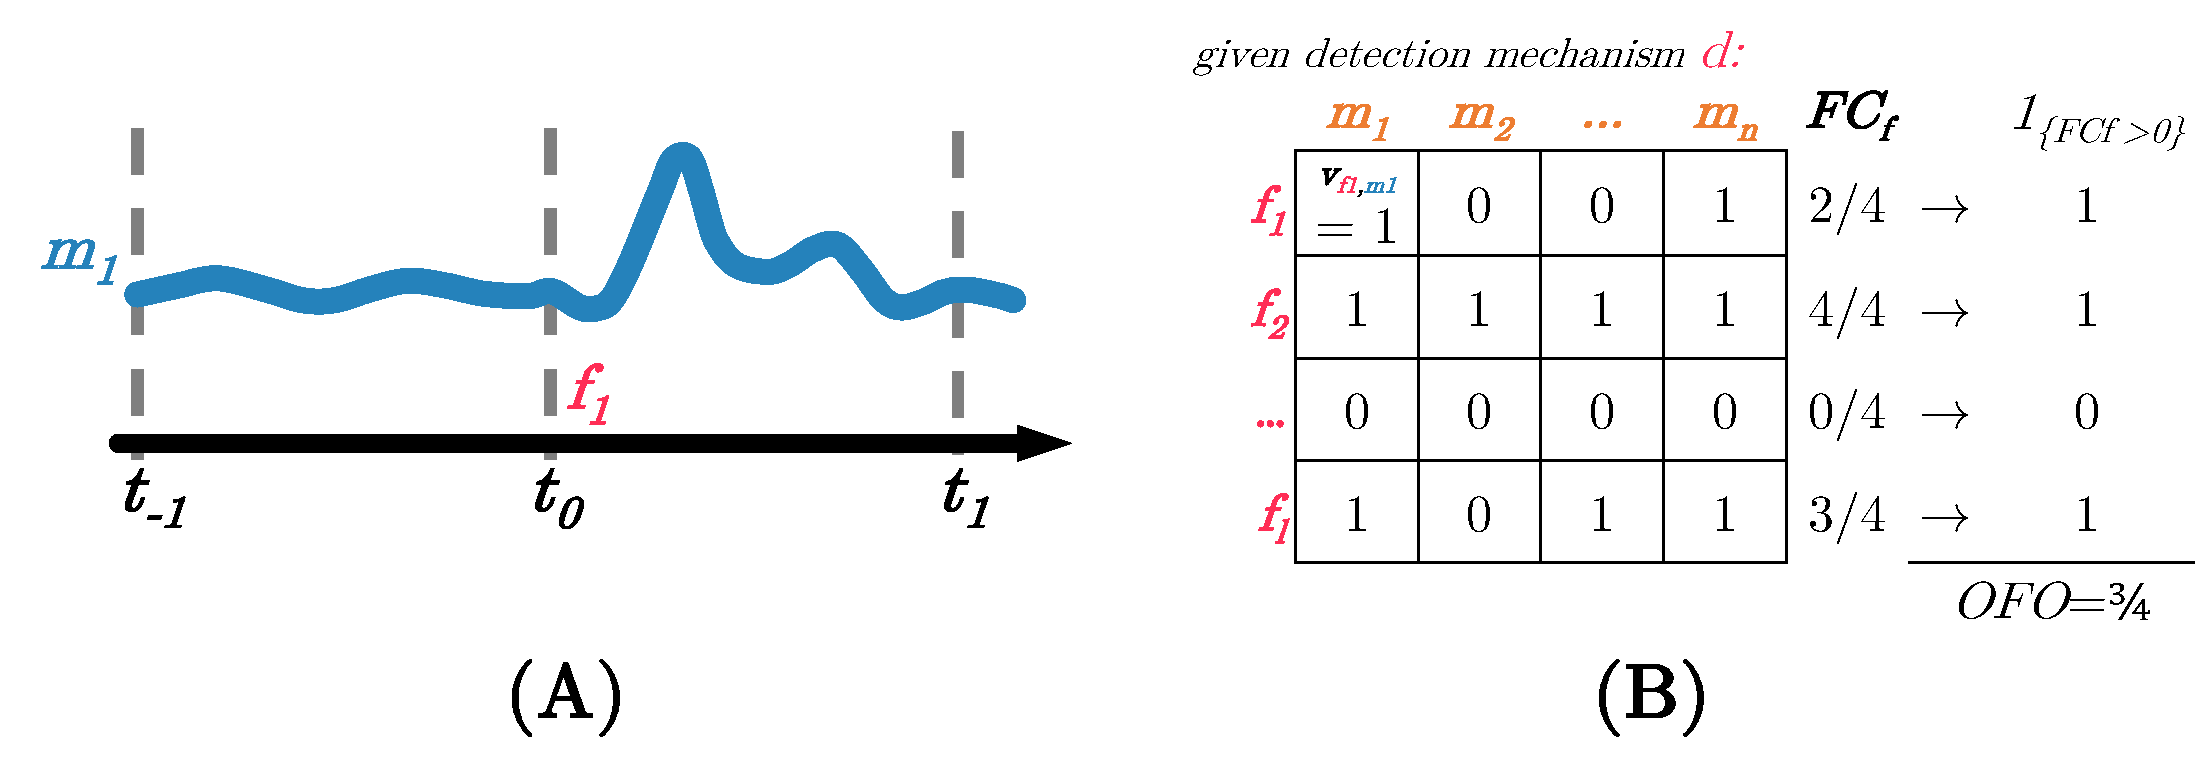
\includegraphics[width=0.9\columnwidth]{figures/fault-model-metricsv4.pdf}
    \caption{(A) Visualization of the fault model, used to define the metrics in (B)}
    \label{fig:faultmodel}
\end{figure}

Figure \ref{fig:faultmodel}(B) illustrates our suggested fault observability metrics using an example. The main goal for developers should be to increase the $OFO$. To achieve this, developers have three options, either increase the visibility of invisible faults by changing the configuration of existing metrics, add additional metrics that are more sensitive to the invisible faults, or make changes to the detection mechanism. 
To weigh between different options, developers need to consider the trade-off between observability overhead and cost. Thus, as a last metric for observability effectiveness, we propose a cost metric. Here, related work \cite{Ernst_OfflineTraceGeneration_2021,Reichelt_OverheadOpenTelemetryEtc,Dinga_EnergyEfficiencyOfMonitoring_2023} has already provided different methods and approaches to quantify the overhead of observability systems. For the purposes of this paper, we will use CPU utilization as a measure for cost, but other metrics such as memory and storage overhead are also suitable.

\subsection{Approach: Observability Experiments}\label{sec:experiments}
We propose an empirical and systematic approach to navigate the observability design space: observability experiments. %
This is a formalized process of experimenting inspired by Chaos Engineering. In Chaos Engineering, faults are injected into a running microservice system to test the system's ability to withstand faults. In our approach, rather than focusing on whether the system survives a fault, we are particularly interested in analyzing the %
quality of observability data generated during such fault experiments. This quality can be quantified with the metrics proposed in the previous section, and can be measured across various observability configurations and instrumentation alternatives. 
Practitioners can use observability experiments as a feedback loop to assess observability design decisions, specifically evaluating which changes in the instrumentation machinery and configuration improve or degrade the metrics, all the while keeping an eye on the cost of these changes.

In the following, we describe the approach briefly. An observability experiment formally consists of a description of the system under experiment (SUE), a workload, a set of treatments and a nonempty set of response variables.

\textbf{System Under Experiment (SUE)} In the context of observability experiments, the SUE is either the entirety of a system or a subset of it, i.e., only a select number of microservices. It is often unnecessary to deploy the entire microservice architecture when developers are only interested in studying the observability and instrumentation of a single service and its dependent services. Therefore, it is important to enable experimentation on subsets, especially considering that modern microservice architectures can quickly grow to hundreds of services \cite{Li_ObservabilityIndustrialSurvey_2022}.

\textbf{Workload} We require load generation to simulate users that create realistic observability data. Because the load can affect the data points of the observability data, we include it as a component of the experiment. Further, as a lot of the metrics devised in the previous section rely on comparative analysis, it is important to also have a way to generate a comparable load repeatedly.

\textbf{Treatments} are controlled changes to the system under experiment. 
Our conceptualization is broader than in Chaos Engineering, where treatment is chaotic or destructive. This need not be the case with treatments in observability experiments. We distinguish between fault treatments and instrumentation treatments. Instrumentation treatments allow users to easily change observability configuration without having to tinker with the SUE code and are executed during compilation. Fault treatments, in turn, are applied at runtime and change the SUE by means of dynamic fault injection.
Treatments allow us to investigate changes to the system typically beyond the scope of Chaos Engineering. For instance, the experiment operator might be interested in investigating if an increase in the sampling interval at some metric instrumentation point results in an increase in accuracy for a fault detection model. %

\textbf{Response Variables} in observability experiments are metrics or distributed traces and represent the different types of observability data that a system can emit. They are used to calculate the fault visibility, fault coverage and overall fault observability. Responses are decoupled from treatments. This means that we can define a response variable that is not directly related to a treatment, i.e., we could observe a response at service A while treating service B. The decoupling allows us to take into consideration higher-order effects of treatments. For example, we might wish to investigate whether injecting a network delay into service A consequently also affects the throughput at other services that depend on A. 

Such experiments are especially feasible in staging environments for systems where both the SUE and the observability system are described using infrastructure as code. In the following, we present a system to automate the process of observability assessments for microservice-based applications.
